\documentclass[journal, a4paper]{IEEEtran}

\usepackage[scheme=plain]{ctex}
% some very useful LaTeX packages include:

%\usepackage{cite}      % Written by Donald Arseneau
                        % V1.6 and later of IEEEtran pre-defines the format
                        % of the cite.sty package \cite{} output to follow
                        % that of IEEE. Loading the cite package will
                        % result in citation numbers being automatically
                        % sorted and properly "ranged". i.e.,
                        % [1], [9], [2], [7], [5], [6]
                        % (without using cite.sty)
                        % will become:
                        % [1], [2], [5]--[7], [9] (using cite.sty)
                        % cite.sty's \cite will automatically add leading
                        % space, if needed. Use cite.sty's noadjust option
                        % (cite.sty V3.8 and later) if you want to turn this
                        % off. cite.sty is already installed on most LaTeX
                        % systems. The latest version can be obtained at:
                        % http://www.ctan.org/tex-archive/macros/latex/contrib/supported/cite/

\usepackage{graphicx}   % Written by David Carlisle and Sebastian Rahtz
                        % Required if you want graphics, photos, etc.
                        % graphicx.sty is already installed on most LaTeX
                        % systems. The latest version and documentation can
                        % be obtained at:
                        % http://www.ctan.org/tex-archive/macros/latex/required/graphics/
                        % Another good source of documentation is "Using
                        % Imported Graphics in LaTeX2e" by Keith Reckdahl
                        % which can be found as esplatex.ps and epslatex.pdf
                        % at: http://www.ctan.org/tex-archive/info/

%\usepackage{psfrag}    % Written by Craig Barratt, Michael C. Grant,
                        % and David Carlisle
                        % This package allows you to substitute LaTeX
                        % commands for text in imported EPS graphic files.
                        % In this way, LaTeX symbols can be placed into
                        % graphics that have been generated by other
                        % applications. You must use latex->dvips->ps2pdf
                        % workflow (not direct pdf output from pdflatex) if
                        % you wish to use this capability because it works
                        % via some PostScript tricks. Alternatively, the
                        % graphics could be processed as separate files via
                        % psfrag and dvips, then converted to PDF for
                        % inclusion in the main file which uses pdflatex.
                        % Docs are in "The PSfrag System" by Michael C. Grant
                        % and David Carlisle. There is also some information
                        % about using psfrag in "Using Imported Graphics in
                        % LaTeX2e" by Keith Reckdahl which documents the
                        % graphicx package (see above). The psfrag package
                        % and documentation can be obtained at:
                        % http://www.ctan.org/tex-archive/macros/latex/contrib/supported/psfrag/

%\usepackage{subfigure} % Written by Steven Douglas Cochran
                        % This package makes it easy to put subfigures
                        % in your figures. i.e., "figure 1a and 1b"
                        % Docs are in "Using Imported Graphics in LaTeX2e"
                        % by Keith Reckdahl which also documents the graphicx
                        % package (see above). subfigure.sty is already
                        % installed on most LaTeX systems. The latest version
                        % and documentation can be obtained at:
                        % http://www.ctan.org/tex-archive/macros/latex/contrib/supported/subfigure/

\usepackage{url}        % Written by Donald Arseneau
                        % Provides better support for handling and breaking
                        % URLs. url.sty is already installed on most LaTeX
                        % systems. The latest version can be obtained at:
                        % http://www.ctan.org/tex-archive/macros/latex/contrib/other/misc/
                        % Read the url.sty source comments for usage information.

%\usepackage{stfloats}  % Written by Sigitas Tolusis
                        % Gives LaTeX2e the ability to do double column
                        % floats at the bottom of the page as well as the top.
                        % (e.g., "\begin{figure*}[!b]" is not normally
                        % possible in LaTeX2e). This is an invasive package
                        % which rewrites many portions of the LaTeX2e output
                        % routines. It may not work with other packages that
                        % modify the LaTeX2e output routine and/or with other
                        % versions of LaTeX. The latest version and
                        % documentation can be obtained at:
                        % http://www.ctan.org/tex-archive/macros/latex/contrib/supported/sttools/
                        % Documentation is contained in the stfloats.sty
                        % comments as well as in the presfull.pdf file.
                        % Do not use the stfloats baselinefloat ability as
                        % IEEE does not allow \baselineskip to stretch.
                        % Authors submitting work to the IEEE should note
                        % that IEEE rarely uses double column equations and
                        % that authors should try to avoid such use.
                        % Do not be tempted to use the cuted.sty or
                        % midfloat.sty package (by the same author) as IEEE
                        % does not format its papers in such ways.

\usepackage{amsmath}    % From the American Mathematical Society
                        % A popular package that provides many helpful commands
                        % for dealing with mathematics. Note that the AMSmath
                        % package sets \interdisplaylinepenalty to 10000 thus
                        % preventing page breaks from occurring within multiline
                        % equations. Use:
%\interdisplaylinepenalty=2500
                        % after loading amsmath to restore such page breaks
                        % as IEEEtran.cls normally does. amsmath.sty is already
                        % installed on most LaTeX systems. The latest version
                        % and documentation can be obtained at:
                        % http://www.ctan.org/tex-archive/macros/latex/required/amslatex/math/



% Other popular packages for formatting tables and equations include:

%\usepackage{array}
% Frank Mittelbach's and David Carlisle's array.sty which improves the
% LaTeX2e array and tabular environments to provide better appearances and
% additional user controls. array.sty is already installed on most systems.
% The latest version and documentation can be obtained at:
% http://www.ctan.org/tex-archive/macros/latex/required/tools/

% V1.6 of IEEEtran contains the IEEEeqnarray family of commands that can
% be used to generate multiline equations as well as matrices, tables, etc.

% Also of notable interest:
% Scott Pakin's eqparbox package for creating (automatically sized) equal
% width boxes. Available:
% http://www.ctan.org/tex-archive/macros/latex/contrib/supported/eqparbox/

% *** Do not adjust lengths that control margins, column widths, etc. ***
% *** Do not use packages that alter fonts (such as pslatex).         ***
% There should be no need to do such things with IEEEtran.cls V1.6 and later.

\usepackage{amssymb}

% Your document starts here!
\begin{document}
\begin{titlepage}

\newcommand{\HRule}{\rule{\linewidth}{0.5mm}} % Defines a new command for the horizontal lines, change thickness here

\center % Center everything on the page
 %----------------------------------------------------------------------------------------
%	LOGO SECTION
%----------------------------------------------------------------------------------------

~\\[1cm]

\includegraphics{SCUT.png}\\[2cm] % Include a department/university logo - this will require the graphicx package

%----------------------------------------------------------------------------------------
%	TITLE SECTION
%----------------------------------------------------------------------------------------

\HRule \\[1cm]
{ \huge \bfseries The Experiment Report of \textit{Machine Learning} }\\[0.6cm] % Title of your document
\HRule \\[2cm]
%----------------------------------------------------------------------------------------
%	HEADING SECTIONS
%----------------------------------------------------------------------------------------


\textsc{\LARGE \textbf{School:} School of Software Engineering}\\[1cm]
\textsc{\LARGE \textbf{Subject:} Electronic and Information}\\[2cm]


%----------------------------------------------------------------------------------------
%	AUTHOR SECTION
%----------------------------------------------------------------------------------------

\begin{minipage}{0.4\textwidth}
\begin{flushleft} \large
\emph{Author:}\\
Weiwen Hu
\end{flushleft}
\end{minipage}
~
\begin{minipage}{0.4\textwidth}
\begin{flushright} \large
\emph{Supervisor:} \\
Mingkui Tan
\end{flushright}
\end{minipage}\\[2cm]
~
\begin{minipage}{0.4\textwidth}
\begin{flushleft} \large
\emph{Student ID:}\\
202021045611
\end{flushleft}
\end{minipage}
~
\begin{minipage}{0.4\textwidth}
\begin{flushright} \large
\emph{Grade:} \\
Graduate
\end{flushright}
\end{minipage}\\[2cm]

% If you don't want a supervisor, uncomment the two lines below and remove the section above
%\Large \emph{Author:}\\
%John \textsc{Smith}\\[3cm] % Your name

%----------------------------------------------------------------------------------------
%	DATE SECTION
%----------------------------------------------------------------------------------------

{\large \today}\\[2cm] % Date, change the \today to a set date if you want to be precise


%----------------------------------------------------------------------------------------

\vfill % Fill the rest of the page with whitespace

\end{titlepage}

% Define document title and author
	\title{Chinese-English Translation Machine Based on Sequence to Sequence Network}
	\maketitle

% Write abstract here
\begin{abstract}
In this experiment we build a sequence to sequence model to do the Chinese-English translation task, with a small-scale open dataset from Tatoeba Project.
\end{abstract}

% Each section begins with a \section{title} command
\section{Introduction}

\PARstart{W}{e} are conducting this experiment in hope of:
1. Understand natural language processing;
2. Understand the classic Sequence-to-Sequence machine translation model;
3. Master the application of attention mechanism in machine tranlstion model;
4. Build machine translation models, verify model performance on simple and small-scale datasets, and cultivate engineering capabilities;
5. Understand the application of Transformer in machine translation tasks.
After the experiment, we get a basic sequence-to-sequence Chinese-English machine translation model. It can successfully translate simple Chinese sentence into English.

% Main Part
\section{Methods and Theory}

\subsection{RNN}

A Recurrent Neural Network (RNN) is a network that operates on a sequence and uses its own output as input for subsequent steps. There are many variants of RNN. In this experiment, we use Gated Recurrent Units (GRUs).

\subsection{The Sequence-to-Sequence Model}

A Sequence to Sequence network, or seq2seq network, or Encoder Decoder network, is a model consisting of two RNNs called the encoder and decoder. The encoder reads an input sequence and outputs a single vector, and the decoder reads that vector to produce an output sequence. As illustrated in figure~\ref{figure:seq2seq}

\begin{figure}[htb]
    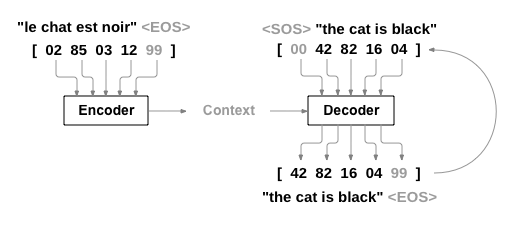
\includegraphics[width=\linewidth]{figures/seq2seq.png}
    \caption{Example of sequence-to-sequence model}
    \label{figure:seq2seq}
\end{figure}

Unlike sequence prediction with a single RNN, where every input corresponds to an output, the seq2seq model frees us from sequence length and order, which makes it ideal for translation between two languages.

With a seq2seq model the encoder creates a single vector $\mathbf{c}\in\mathbb{R}^N$ which, in the ideal case, encodes the “meaning” of the input sequence into a single vector.

\subsection{Attention in Decoder}

If only the context vector $\mathbf{c}$ is passed betweeen the encoder and decoder, that single vector carries the burden of encoding the entire sentence.

Attention allows the decoder network to "focus" on a different part of the encoder’s outputs for every step of the decoder’s own outputs. First we calculate a set of attention weights. These will be multiplied by the encoder output vectors to create a weighted combination. The result should contain information about that specific part of the input sequence, and thus help the decoder choose the right output words.

Calculating the attention weights is done with another feed-forward layer, using the decoder’s input and hidden state as inputs. Because there are sentences of all sizes in the training data, to actually create and train this layer we have to choose a maximum sentence length (input length, for encoder outputs) that it can apply to. Sentences of the maximum length will use all the attention weights, while shorter sentences will only use the first few.

The \emph{dot-product} attention is also very famous. It don’t have restriction on input length, and is used by the \emph{Transformer} models. We don’t use this type of attention is this experiment though.

\section{Experiments}

\subsection{Dataset}

We use the Chinese-Engilish bilingual sentence pairs from \emph{Tatoeba Project}\footnote{https://www.manythings.org/anki/cmn-eng.zip}. It consists of 24,026 pairs. Since the dataset is small, the model is not likely to learn very complex translation. So I just used the pairs with Chinese sentence shorter than 16 characters. I randomly choose 70\% (15,802 samples) for training and use the rest (6,773 samples) for testing.

\subsection{Implementation}

I use PyTorch to implement the model and the whole pipeline. Although I referred to the official tutorial\footnote{https://pytorch.org/tutorials/intermediate/seq2seq\_translation\_\\ tutorial.html}, there are still some major differences:
First, My model can process a batch of sentence pairs, which greatly improves the training efficency. And this should also improve the training result stability, since we can use mini-batch SGD to work with more accurate gradient.
Second, I implemented a slightly more complicated tokenizer, which can handle punctuations, and some more special cases.
Last, My pipeline is fully distributed. It can utilize multiple GPUs to accelerate the training.

For Chinese sentence tokenization, I just split each character as a token. And I also did some normalization on punctuations.

The BLEU Implementation is from torchtext package.

All parameters are initialized using default method in PyTorch. I use Adam optimizer with default parameters (learning rate 1e-3, $\beta$ 0.9, 0.999) other hyper-parameters are summarized in table~\ref{table:hyper-param} The whole training process only takes 3 minutes on 2 GeForce GTX TITAN X GPU.

\begin{table}[htb]
    \centering
    \caption{Hyper Parameters}
    \label{table:hyper-param}
    \begin{tabular}{l|r}
        \hline
        Epoch         & 50  \\
        Batch size    & 512 \\
        Dropout       & 0.1 \\
        Encoder hidden size & 512 \\
        Decoder hidden size & 512 \\
        \hline
    \end{tabular}
\end{table}

\subsection{Results}

The experiment result is summarizes in table~\ref{table:results}

\begin{table}[htb]
    \centering
    \caption{Results}
    \label{table:results}
    \begin{tabular}{l|rr}
        \hline
                    & Train  & Test \\
        \hline
        loss        & 0.0433 & 6.8399 \\
        token accuracy (\%) & 98.79 & 34.54  \\
        BLEU        & -      & 0.2011
    \end{tabular}
\end{table}

Very different from the previous linear classification experiment, this experiment shows severe overfitting. As illustrated in figure~\ref{figure:loss} and figure~\ref{figure:acc}, The training loss is 2 orders of magnitude smaller than the test loss, and the token accuracy on training samples is nearly 100\%. This could be because the model is more complicated, and is capable to "remember" all training samples; and because the translation task is more complicated while the amount of training data is too few.

\begin{figure}
    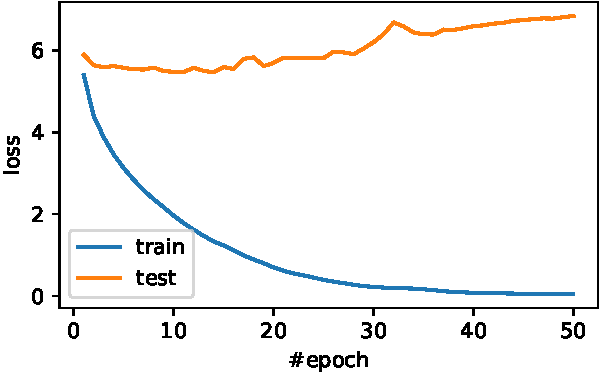
\includegraphics[width=\linewidth]{figures/loss.pdf}
    \caption{Loss change with number of epoch}
    \label{figure:loss}
\end{figure}

\begin{figure}
    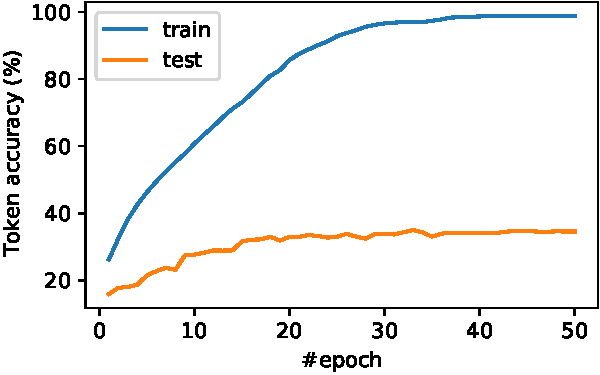
\includegraphics[width=\linewidth]{figures/acc.pdf}
    \caption{Token accuracy change with number of epoch}
    \label{figure:acc}
\end{figure}

Here I show some of the translation results in test set:

Success samples:

\begin{itemize}
    \item 湯姆拍了手。\newline tom clapped .
    \item 你喜歡這些照片里的任何一張嗎?\newline
    do you like any of these pictures ?
    \item 請進來。\newline please come in .
\end{itemize}

Not accurate but make some sense:

\begin{itemize}
    \item 他偷了她的手表。\newline he had her arm .
    \item 這不便宜, 是嗎?\newline it 's not warm , isn't it ?
    \item 我们现在就去医院吧。\newline let 's go out the right away .
\end{itemize}

Failure samples:

\begin{itemize}
    \item 参见上文。\newline the man to the tree .
    \item 你的包开着。\newline your team is right .
    \item 雪停了。\newline it 's 3:30 .
\end{itemize}

Some failure is caused by perticular words not recognized by the model, the overall sentence structure is fine. But there are also some failures not making any sense to me.

\section{Conclusion}

This experiment gives satisfying results. The 3-minute training and 1.6k training bilingual sentence pairs give a not-so-bad machine translation model. It can handle simple sentences. In this experiment, I'm familiarised with the sequence-to-sequence model as well as other parts of the machine learning pipeline. And my engineering skills are improved.

\end{document}
